\documentclass[a4paper, 12pt, singlepage]{report}

\usepackage[utf8]{inputenc}
\usepackage[T1]{fontenc}
\usepackage[acronym]{glossaries}
\usepackage{graphicx}
\usepackage{booktabs}
\usepackage{pdfpages}
\usepackage{hyperref}
\usepackage{listings}
\usepackage{tablefootnote}
\usepackage{verbatim}
\usepackage{multirow}
\usepackage{subcaption}
\usepackage{floatrow}
\usepackage[binary-units=true, per-mode=symbol]{siunitx}
\usepackage{wasysym}
\usepackage{physics}
\usepackage{hyperref}

\usepackage[numbers]{natbib}

\title{Kernel Bypass for fast replicated RPCs }
\author{Antoine Albertelli}
\date{Fall semester, 2018}

\newacronym{r2p2}{R2P2}{Request Response Pair Protocol}
\newacronym{nic}{NIC}{Network Interface Card}
\newacronym{rpc}{RPC}{Remote Procedure Call}
\newacronym{dcsl}{DCSL}{Data Center Systems Laboratory}
\newacronym{ssd}{SSD}{Solid State Disk}

\lstset{language=C++,frame=single}

\newfloat{lstfloat}{htbp}{lop}
\floatname{lstfloat}{Listing}
\def\lstfloatautorefname{Listing} % needed for hyperref/auroref

\begin{document}

\setcounter{tocdepth}{1}

\maketitle

\tableofcontents

\chapter{Introduction}

motivation (why does consensus matter in dc systems)

prob. statement (what if consensus was in the transport instead of the application?)

hint of the solution (consensus as part of the transport for rpcs)

enumerate contributions (raft as part of transport)

killer numbers

skeleton of the thesis


\chapter{Background}
\label{chap:background}

\section{Distributed Consensus}

% large system -° failures will occur
% somehow need to be reliable in the face of such problems
When scaling out to large number of nodes, the likelihood of a node failing increases.
Therefore, we would like the aggregate system to stay operational despite the failures of individual nodes.
A very useful primitive to reach this property is called \emph{distributed consensus}, which provides the cluster with a way to agree on a value, despite individual failures.

This primitive can then be extended using asynchronous state machine replication.
In this model, the values are instructions executed by a state machine running on each node.
Since the initial state is specified, and all nodes in the cluster execute the same operations in the same order, we know that the state on every node after $i$ instruction will be the same.
Note that not all nodes might reach a given instruction at the same time.
For example, a node separated from the peers by a network failure can not receive the latest update; it will catch up later, when connectivity is restored. 
However, once a value was chosen by the cluster, we know for sure that this value will eventually be accepted by all nodes. 
In other words, it is not possible for a node to change already-made decisions. 

Typical replication protocols provide $2n + 1$ replication, meaning a cluster can stay alive as long as a majority of nodes is alive.
For example, if there is 5 nodes in the cluster, up to two could go offline without impacting the availability or the consistency of the data.
While it might seem like a good idea to make extremely large clusters, each additional node will increase the network load.
A trade off between reliability must, again, be made here.

An important restriction to make is the type of node failures that we are concerned with.
We will be using the \emph{non-byzantine} model of failures\cite{paxos_made_simple}, in which the following properties hold.
First, nodes may fail by stopping, and may restart (note that this requires persistent storage in case all nodes die).
In particular, nodes are assumed to be non-malicious and non-bogus.
Then, messages can be re-ordered, can be duplicated, lost or delayed, but they cannot be corrupted.
Dealing with those types of failure (especially malicious nodes) require a different set of algorithms, with much less performance.

\subsection{Raft Consensus Protocol}

Raft\cite{raft} is a protocol that proposes a solution to the distributed consensus problem.
Its main goal is to be easy to understand while still being efficient.
It achieves its objective by cleanly separating different concerns of the protocol.
It also provides a strong leader, \ie all entries flow from the leader to the followers, making it simpler to reason about.
Unlike the original Paxos, Raft provides a complete solution to build a replicated log.


\begin{figure}[h]
    \centering
    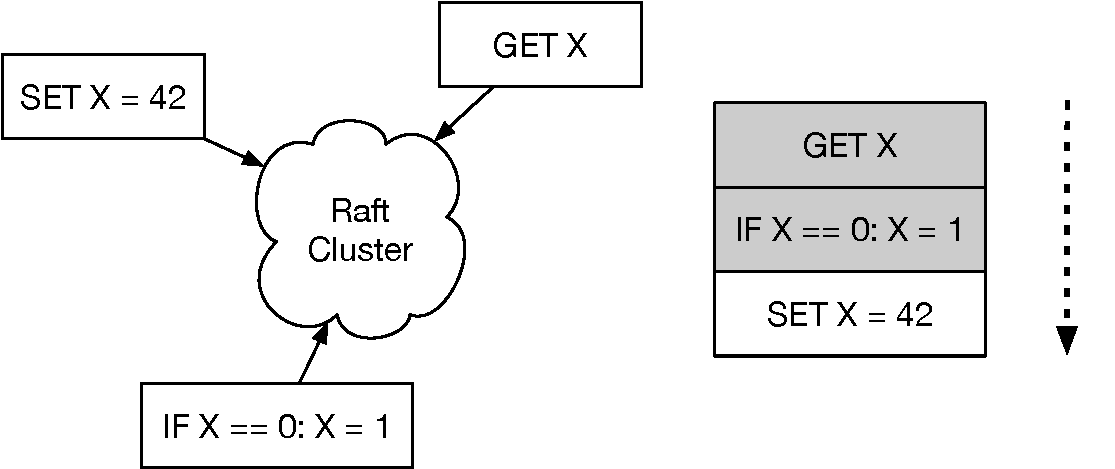
\includegraphics[width=0.8\textwidth]{replicated_log}
    \caption{Example asynchronous operations for a simple key value store supporting atomic compare and swap operation.
        Also shown on the right is the replicated log.
        Entries in grey are committed, meaning they will never be overwritten, while the last one cannot be assumed to be persistent yet.
    \label{fig:replicated-log}
    }
\end{figure}

The approach chosen by Raft to model the consensus protocol is called a \emph{distributed log}.
Under this approach, the values replicated by Raft are put inside a queue called the log (Figure~\ref{fig:replicated-log}).
Raft then replicates the log on all nodes, and guarantees that all the logs in the cluster will have the same operations in the same order.
Raft also keeps track of which entries are replicated on every node.
Once an entry has been replicated on a majority of machines, Raft guarantees it will never be removed from the log again.
Such entries are called \emph{committed}.
Raft log entries can be used as instruction to implement a replicated state machine.

Raft can be split in three different parts: leader election, log entries replication and commit propagation.
Each node can be in one of three states: \emph{follower}, \emph{candidate} or \emph{leader}.
During normal operation (when a leader emerged), a cluster contains exactly one leader and zero candidates.
We will start by assuming that everything is normal to explain how the protocol works, then explain what changes during leader election.

But before we must introduce an important Raft concept called the \emph{term}.
One term is defined as a period of time in which there is at most one leader.
This means that in order to change the leader, a new term must be changed.
Terms are identified by their term number, which always increases.
Note that not all terms have leader, for example if no leader could be elected, the term number is increased before starting a new round of elections.

\subsection{Log Replication}

When the leader receives a request from a client, it appends it to its local log, tagging it with its index (a monotonic entry counter) and term number.
It will then periodically send \emph{AppendEntries} requests to the followers.
Each of those contains all the entries that were not yet acknowledged by the destination follower.
It also contains the term and index of the entries immediately before the first one in the request.
This allows a follower to detect any gap between its local log and the incoming entries.

The destination follower will then append the new entries contained in the \emph{AppendEntries} request to its own log.
During this step, the entries' terms and indices are used to detect inconsistencies and duplicated entries.
It then sends a reply to the leader to acknowledge that the incoming entries were correctly replicated.
It can also notify the leader of a failure to replicate, for example due to a gap in the log.

Note that the checks performed when processing \emph{AppendEntries} requests guarantee that, if two log entries on two different machines have the same index and term, then two properties must hold\cite{raft}.
First, the two entries must store the same content.
Then, all previous log entries are also matching between the two logs.
Those consistency properties allow Raft to have a simpler entry committing mechanism.

\subsection{Entries commit}

We say that an entry is \emph{committed} when we know for sure that this entry will never be lost by the cluster.
We also know that a committed entry will eventually be replicated to the whole cluster.
This means that to be committed, an entry must be replicated on a majority of servers.
When an entry is marked as committed, its content can be consumed by the application.

Raft does not keep track of the commit status for each individual entry.
Instead, it tracks the last committed entry; all entries before are considered committed too.

The leader keeps track of the latest acknowledged entry for each follower.
Once an entry has been replicated on a majority of machines, the leader moves its commit index to it.
The followers are then told to update their local commit status to the new index.

\subsection{Leader Election}

In Raft, leader election is based on timers.
First, a periodic timer is used by the leader to send heartbeats to followers.
Those heartbeats are \emph{AppendEntries} requests, which can be empty if there is no new request to replicate.
Every time one of those heartbeats is received, the follower resets the second timer, called the \emph{election timeout} timer.

If no messages is received from the leader, then the election timer will fire.
The follower can then then start a new leader election.
It will first increment the term, as there can be only one leader per term.
It will then transition to the candidate state and send \emph{Vote} requests to other cluster participants.

Once a node receives a \emph{Vote} request, it decides wether or not to grant its vote to the requesting candidate.
To do so, it will first check that the candidate's term is more recent than its own.
It will also check that the candidate's log is at least as complete as its own.
This ensures that the leader's log contains all committed entries.
If this was not the case, then the leader would start replacing committed entries, leading to loss of consistency.
Finally, the node sends a reply to the candidate containing the status of its vote.

If a candidate reaches majority, then it transitions to the leader role and starts sending heartbeats.
Otherwise, the election timeout will fire again, restarting the process at a new term.
To avoid conflicting elections where no majority can occur, the timeout duration is randomized, so that election will eventually succeed.


\begin{figure}[h]
    \centering
    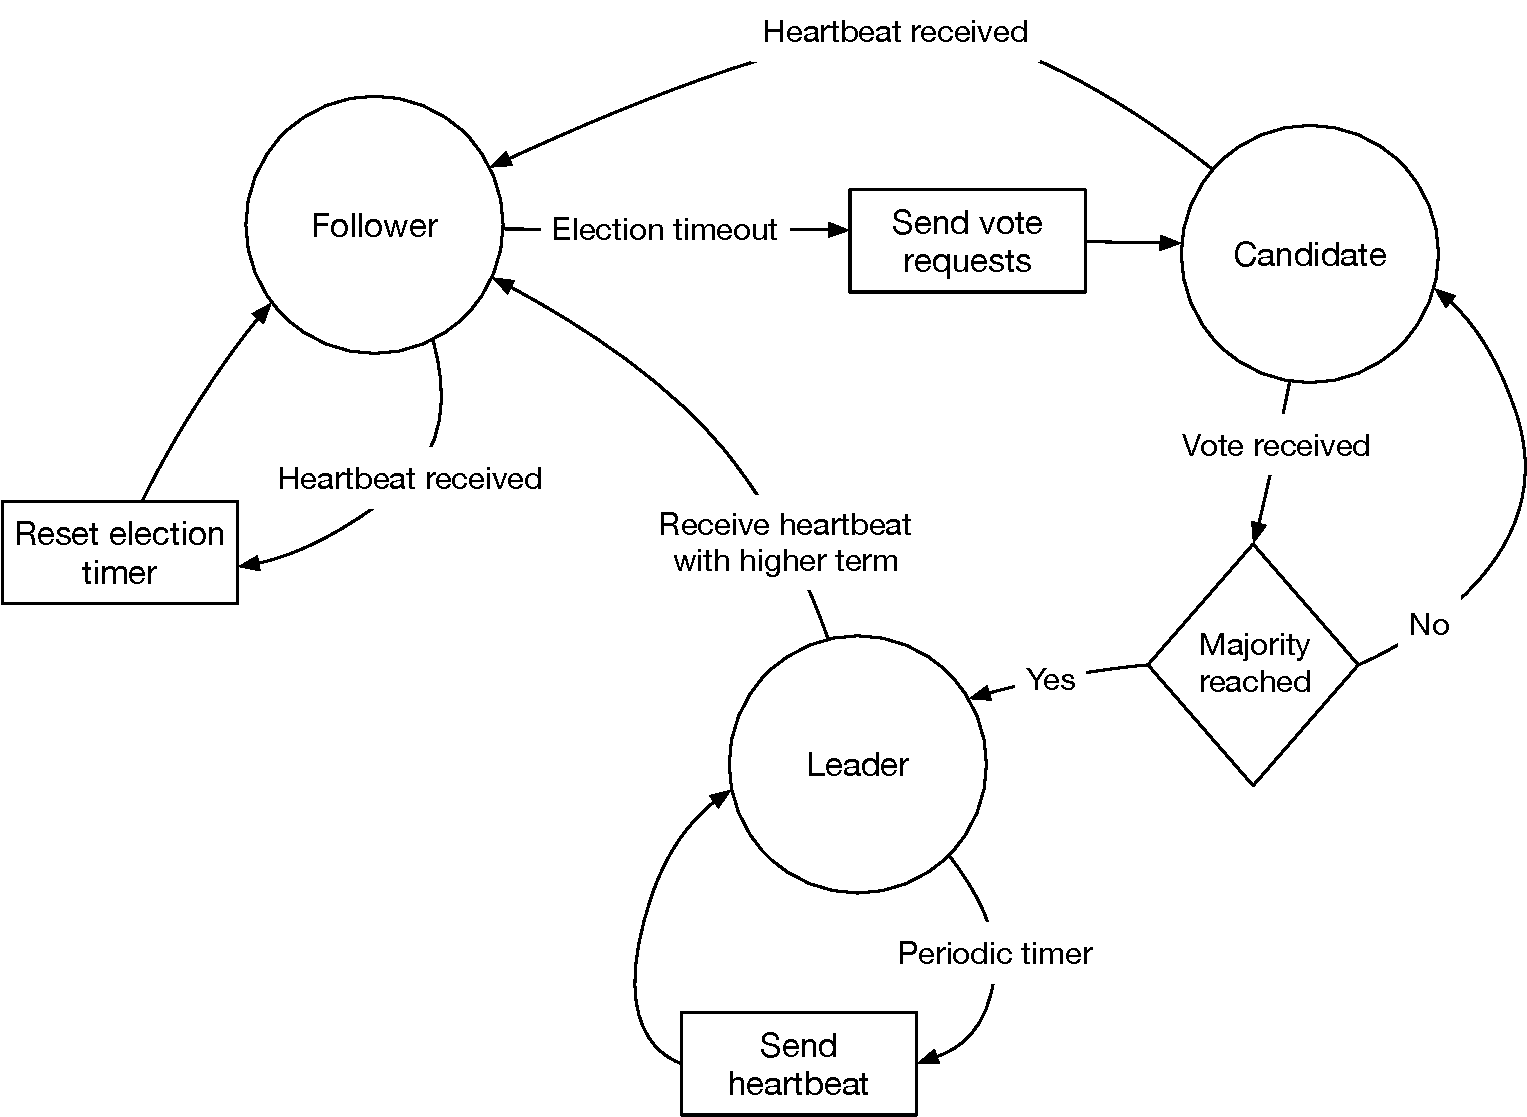
\includegraphics[width=0.8\textwidth]{raft_states.pdf}
    \caption{Raft node state machines showing leader election logic.
    \label{fig:raft-leader-election}
    }
\end{figure}


\section{Transport protocols}

% what is a transport protocol
%   Part of the internet infra
%     provides many functionalities: multiplexing, congestion control, reliable delivery, connection establishement, etc
%     handles delivery of the data to the application

Transport protocols build on the the network (IP) layer and provide services to the applications.
The most important service is multiplexing; several application can use the network, and the transport routes information to them.
This is done using port numbers.
Historically, IP was used with two transport protocols: UDP and TCP.

While UDP only provides connection multiplexing, TCP is much more complicated.
It provides a stream interface, which guarantees that bytes that enter the connection will arrive in the same order at the other end (reliable delivery).
In order to do so, TCP uses has to establish a connection and then acknowledge packets.
It also provides congestion control functionality to avoid link saturation.

All those features made TCP the logical choice when sending data on the Internet, which is pretty unreliable.
However, when running inside a datacenter, packet loss or re-ordering is not as likely.
In addition to this, TCP connection tracking requires requires a lot of messages to send some data, increasing latency (Figure~\ref{fig:tcp_lifecycle}).

%
% historical: tcp and udp
%     nowadays hard to change this due to things such as nat
%
% new protocols such as quic and
%
% need for a RPC protocol, lots used HTTP
%
% connection handshake: maybe a tcp connection establishment diagram ?


\begin{figure}
    \centering
    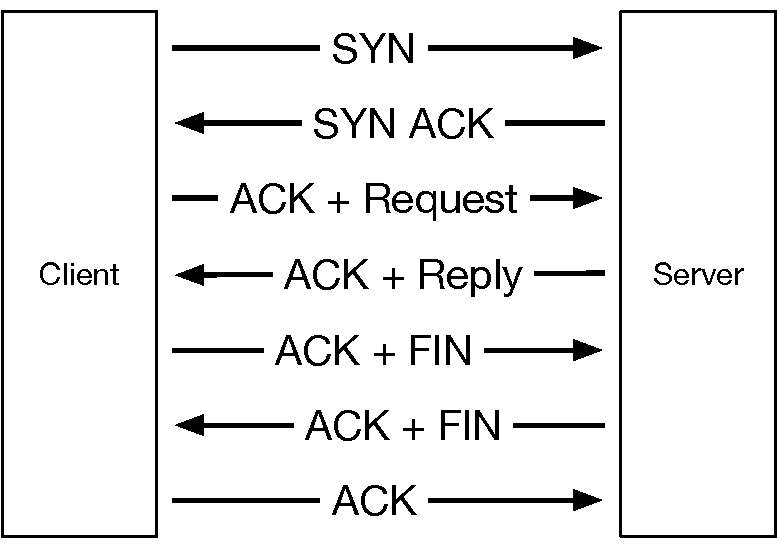
\includegraphics[width=0.4\textwidth]{tcp_lifecycle}
    \caption{Lifecycle of a typical \gls{rpc} over TCP (such as HTTP) interaction.
        We see that the latency before the reply is available takes at least two \gls{rtt}.
    \label{fig:tcp_lifecycle}
    }
\end{figure}


\subsection{Request Response Pair Protocol (R2P2)}

Most current \gls{rpc} systems, such as Google's gRPC\cite{grpc} or Facebook's Thrift\cite{thrift} typically use TCP as their transport layer.
In order to address TCP's shortcomings, the \gls{dcsl} developped a new transport protocol specially designed for \glspl{rpc}.
Unlike TCP, this new protocol is connectionless; each communication is made of a single request followed by a single response, hence the name of \gls{r2p2}.
This reduces latency by removing the handshake \gls{rtt} of TCP.

\Gls{r2p2} has been succesfully used in the past to implement new load balancing techniques\cite{r2p2}.
Since it was designed with load balancing, each \gls{r2p2} request includes includes a field to specify how it should be routed.
For example, it can be marked as ``Fixed'', meaning that the request must be served by the receiver, or ``load-balanced'', in which case the router is free to redirect it to another server.
Since \gls{r2p2} has no notion of connections, the reply can be sent directly to the client instead of having an additional trip through the load balancer (Figure~\ref{fig:load_balancing}).

\begin{figure}
    \centering
    \begin{subfigure}[t]{0.4\textwidth}
        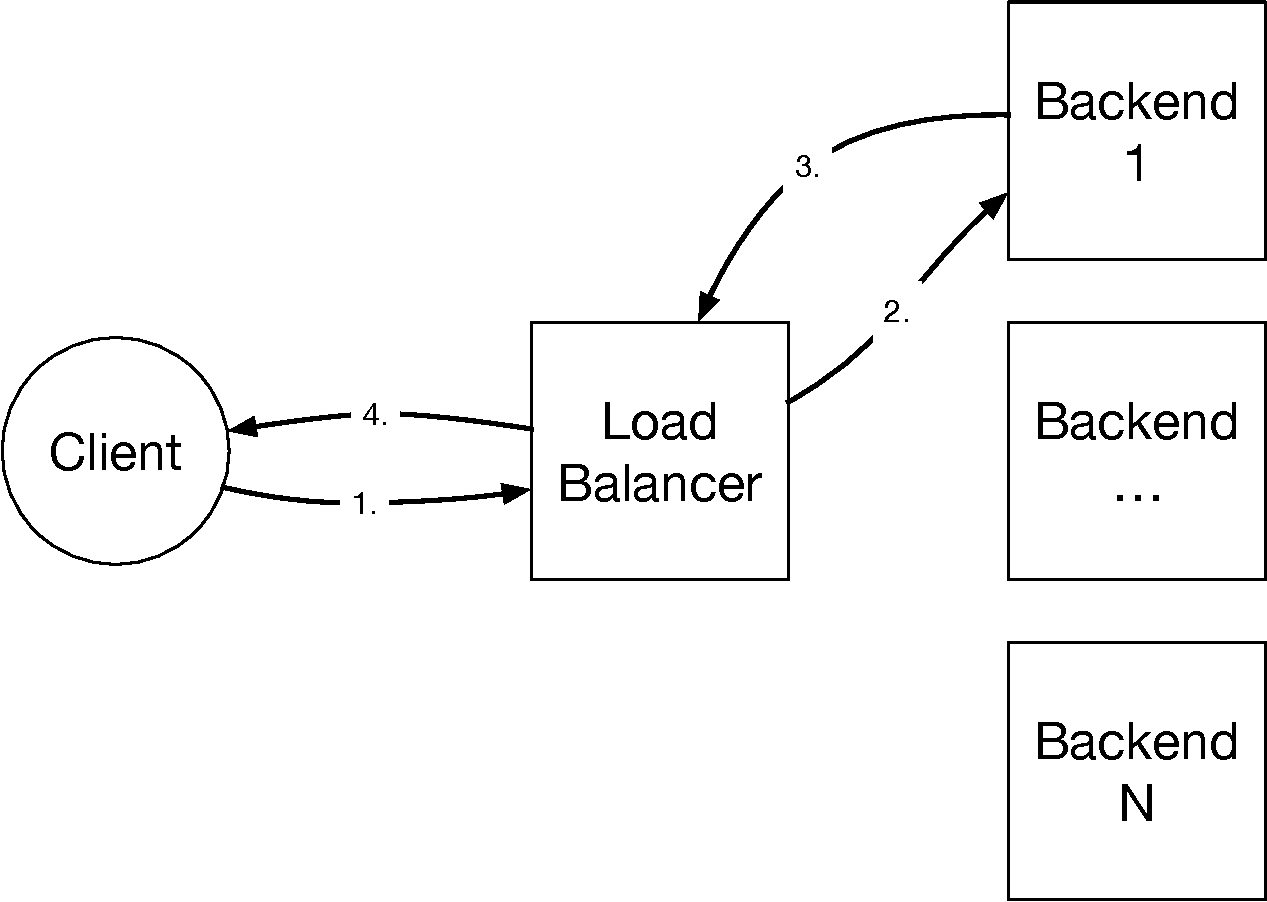
\includegraphics[width=\textwidth]{load_balancer_interaction_tcp.pdf}
        \caption{TCP}
    \end{subfigure}%
    ~
    \begin{subfigure}[t]{0.4\textwidth}
        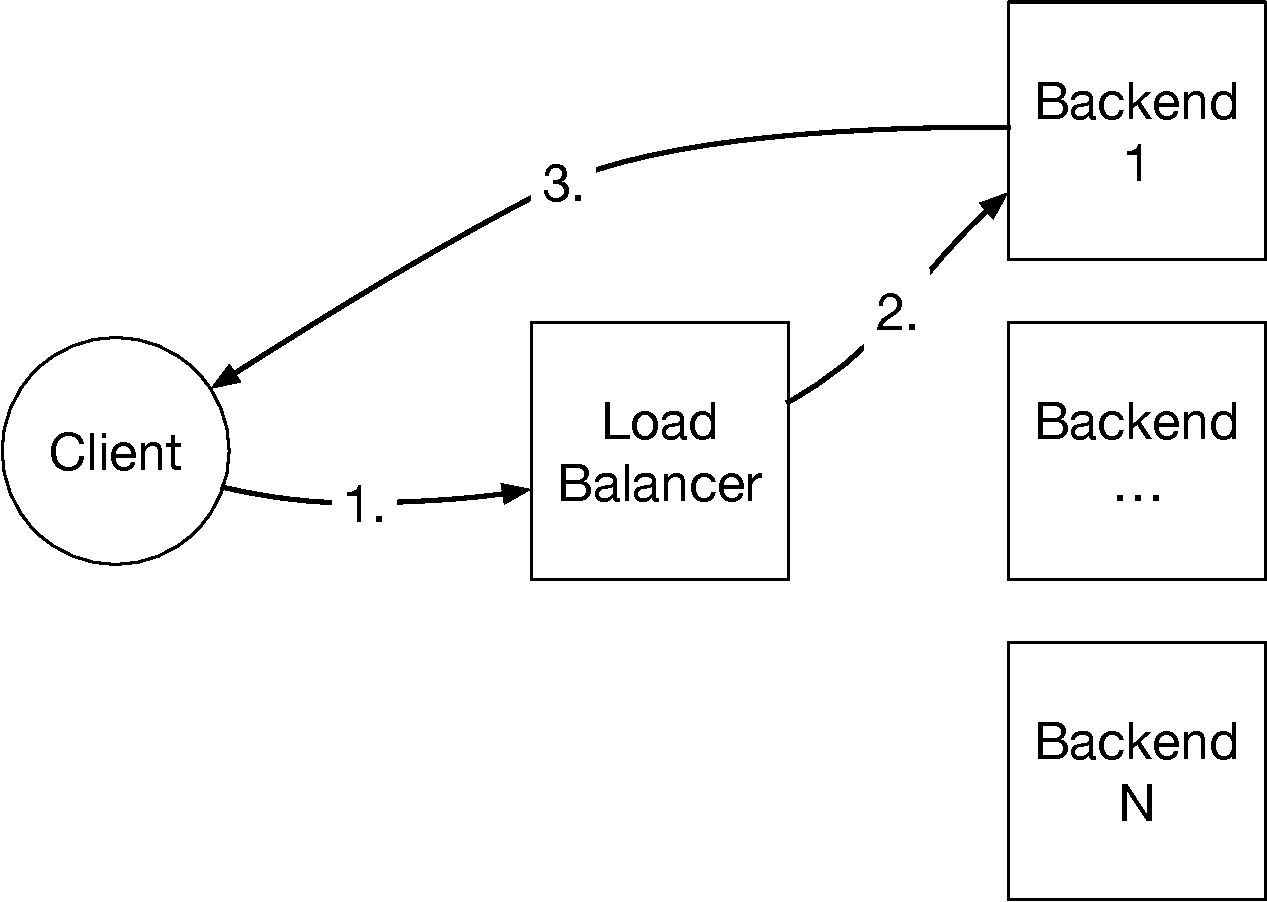
\includegraphics[width=\textwidth]{load_balancer_interaction_r2p2.pdf}
        \caption{\gls{r2p2}}
    \end{subfigure}
    \caption{
        Load balancing data flow using both TCP and \gls{r2p2}.
        We can see that the connection-less nature of \gls{r2p2} allows data to be sent directly back to the client.
        \label{fig:load_balancing}
    }
\end{figure}


We realized that it could be interesting to embed the replication mechanism in the transport layer.
This would greatly simplify the life of the application developer.
Any networked application can be turned into a replicated version of it simply by changing a flag on the requests.
Clients could even choose wether or not to ask for replication based on application-specific logic.
For example, if stales read from a key-value store are acceptable, read request could be marked as ``load-balanced'', while write requests would be marked as ``replicated'' to ensure consistency.


\subsection{R2P2 API}

The \gls{r2p2} library \gls{api} looks nothing like a BSD socket \gls{api}.
Instead it is \emph{event oriented}: the user of the library provides a set of callbacks that are called when a request is received (in the case of a server) or when a response arrives (in the case of a client).
Those callbacks also receive a per-connection argument which can be used to track state.
The core of the \gls{r2p2} \gls{api} can be seen in Listing~\ref{listing:r2p2-client-api} and \ref{listing:r2p2-server-api}.

Such event-oriented \gls{api} maps well to the semantics of either high performance I/O syscalls (\eg Linux's \texttt{epoll}) or the one of kernel bypass frameworks such as DPDK.

\begin{lstfloat}
\lstinputlisting[label=listing:r2p2-client-api,caption={\gls{r2p2} \gls{api} summary}]{code_snippets/r2p2_client_api.c}
\end{lstfloat}

\begin{lstfloat}
\lstinputlisting[label=listing:r2p2-server-api,caption={\gls{r2p2} server \gls{api}}]{code_snippets/r2p2_server_api.c}
\end{lstfloat}

With our proposal of bringing the consensus protocol to the transport layer, switching a normal application to a distributed, consistent one is simply a matter of changing the \texttt{routing\_policy} field from \texttt{FIXED\_ROUTE} to \texttt{REPLICATED\_ROUTE}.
We hope that this will create a re-usable framework and that more developper will be able to write fault tolerant systems as a result.

\section{Kernel Bypass}

Due to the way time sharing operating system work, switching between userland and kernel code, or between two userland tasks is expensive (about \SIrange{1}{2}{\micro\second}\cite{measuring_context_switch})..
This is due to the need of saving the whole original execution context first, and then loading or restoring the new execution context.
Since every system call switches to kernel code, high performance code can be severly limited by the amount of syscall it is doing.
For example, assume that a simple packet forwarding application running on Linux uses one syscall to read a packet, and another syscall to write it again.
This means up to \SI{4}{\micro\second} of context switching per packet, restricting performance to about \SI{250}{\kilo packet\per\second}.

Another important optimization used by high performance networking code is to avoid using interrupts.
Interrupts are a way for a peripheral, such as a \gls{nic}, to notify the main processor, for example when an incoming packet is ready for processing.
They allow the processor to avoid checking the presence of processing tasks needlessly, saving computational power and energy.
However, they are also quite slow to be processed, increasing latency.
In high packet rate applications, a processor can safely assume that a packet will always be available, or just check again if this is not the case.
The loss in energy or power is quite low, and the gain in throughput and latency significant.
By removing context switches and interrupts, Google observed a 3x gain in throughput\cite{maglev}.

To reduce the number of switches between kernel space and userland, we have two choices.
The first would be to move moving more parts of the system in the kernel, while the second moves more parts of the system to userland.
The first option is the one that has been traditionnaly been used for networking; the TCP/IP stack or the filesystem are part of typical UNIX kernels.
This technique is very efficient in terms of developper efforts; by using the kernel-provided facilities, engineers gain access to a high-quality implementation shared by many users.
However, moving application-specific code in kernel space is not an easy task.
This is due to the usual challenges of kernel development: very little memory protection, lack of debugging tools, possibility to crash the development machine if testing on it, \etc
The lack of memory protection for kernel code also opens the door to security vulnerabilities, which can be pretty severe when processing network traffic.
While modern operating systems offer security features to mitigate this risk\cite{kernel_self_protection}, writing correct kernel code is still a difficult exercise.
This is made even more difficult by the fact that Linux's internal \gls{api} are considered unstable by developpers.
This means that applications may break as kernel gets updated, making maintenance more expensive than expected.

For all these reasons, modern high performance systems tend to move more, if not all, of the processing application in userland, as part of the application.
This technique is known as \emph{kernel bypass}, because it bypasses the kernel to talk to the underlying hardware directly.
In this approach, the application embeds everything it needs, from \gls{nic} drivers to TCP.
While writing a \gls{nic} driver might seem like a waste of developer's time, one generally uses framework and libraries to implement this functionality.
The main downside of \emph{kernel bypass} is that it prevents sharing of ressources between applications running on the server.
For example, each networked application would need its own \gls{nic}, which can be an issue in a commercial cloud environment.
It is also more complicated to develop, and therefore reserved for performance sensitive applications. 

A key contribution of our work is the use of kernel bypass techniques to reduce latency.
In particular, we are opposing our design to Kernel Paxos\cite{kernelpaxos}, which moved the Paxos consensus protocol in the Linux kernel with great results.
We believe that using kernel bypass techniques can lead to similar, if not better performance without compromising process separation.

\chapter{Design}
\label{chap:design}

\section{Choice of a consensus protocol}

One of the earliest solution to the consensus problem is Lamport's Paxos algorithm\cite{paxos}.
It is currently widely used, for example Google relies on it to ensure correctness of its distributed systems\cite{chubby, paxoslive}.
However, Paxos has two issues: first, it only solves part of the problem; some other ``bricks'' must be added to it to form a complete system.
In addition to this, Paxos is known to be hard to understand, and even harder to implement correctly.
Most of its users rely on pre-existing implementations such as libpaxos\footnote{\url{https://bitbucket.org/sciascid/libpaxos/}}.
This means modifying the consensus protocol for our application and chosen transport could be hard to do

Fortunately for us, a simpler alternative to Paxos called Raft was recently introduced\cite{raft}.
Raft was designed from the ground up to be simpler by cleanly separating the different parts of the problem.
It also provides a complete solution, unlike Paxos which often requires additional, unproven extensions\cite{paxoslive}.

Another possible choice would have been ZooKeeper's ZAB\cite{zookeeper}, but it was not as well documented as Raft.
In addition, it appeared to provide primitives that were less general purposes than a replicated log.

Despite the availability of excellent production grade Raft implementations, we decided to implement our own.
Most existing Raft implementations are using high level languages such as Go, which are not suited for low latency programming.
Other implementations in C or C++ make a lot of assumptions on the underlying platform.
For all those reasons, it was deemed easier to do it ourself, using experience gathered by doing a prototype in Python.
The resulting implementation is pretty small, at about 1000 lines of C++ code.

\section{Modifications to R2P2}


\begin{figure}
    \centering
    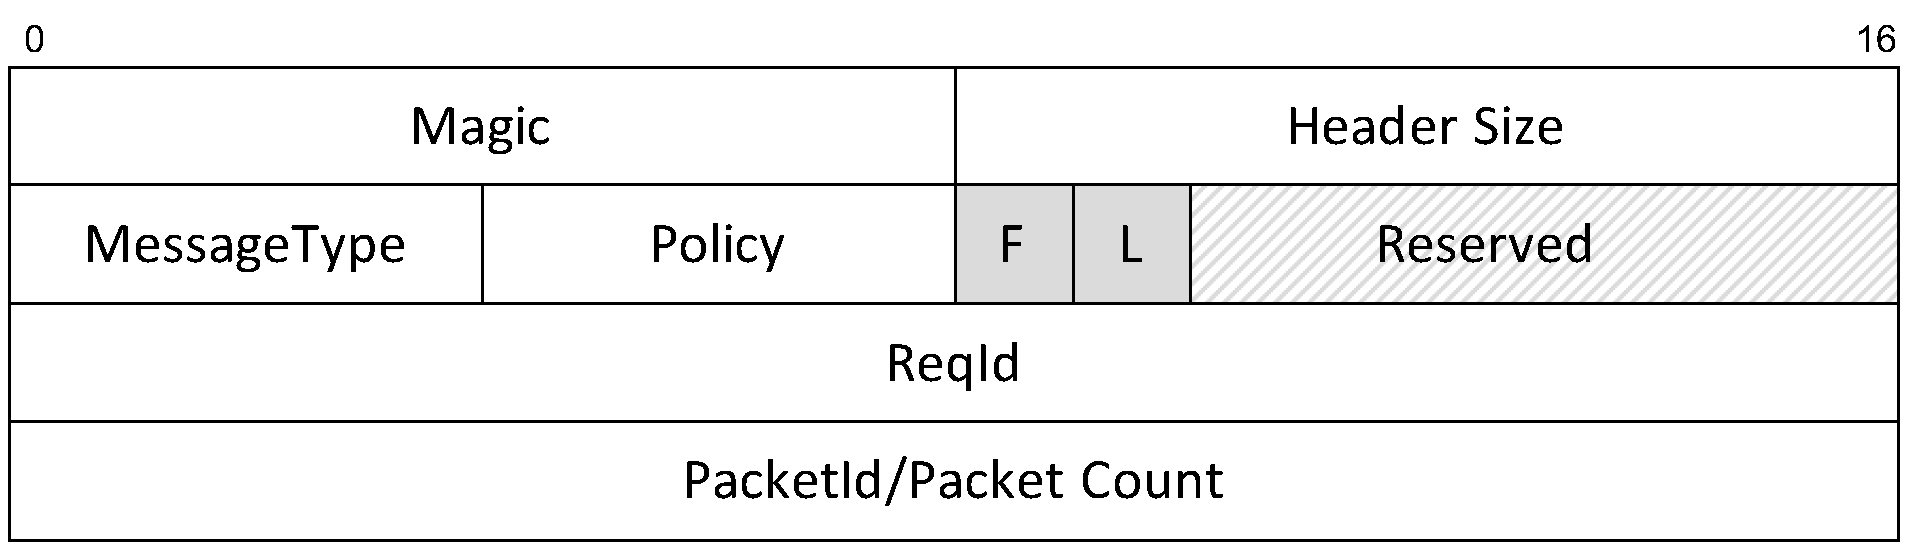
\includegraphics[width=0.6\textwidth]{r2p2_header}
    \caption{\gls{r2p2} header format\cite{r2p2}}
    \label{fig:r2p2-header}
\end{figure}


\Gls{r2p2} requests have a \emph{Policy} field to indicate to load balancers how this request should handled (Figure~\ref{fig:r2p2-header}).
The pre-existing policies were \texttt{LB\_ROUTE} (can be redirected to any backend) or \texttt{FIXED\_ROUTE} (the request should really be handled by the destination backend).
We added the \texttt{REPLICATED\_ROUTE} policy: all the backends will eventually receive this request.
In addition, all backends are guaranteed to receive the requests using this policy in the same order.

Since this policy field is per request, it means clients can selectively enable request replication.
For example, a user might specify that no write should be lost but that stale reads are acceptable (to lower latency).
Then write requests would be sent with the \texttt{REPLICATED\_ROUTE} policy, while reads are sent with \texttt{LB\_ROUTE}.

Another addition to the R2P2 protocol was to add a new \emph{MessageType} for Raft-related messages.
The different types of Raft messages are differentiated in the \gls{r2p2} payload using a type field.
The list of messages and their description can be found below.
In addition, each message contains the term number of the sender, as it is required for all Raft operations.

\begin{description}
    \item[VoteRequest] Fields: \texttt{last\_log\_index}, \texttt{last\_log\_term}.
        Sent from one candidate to a follower to request a vote for itself.
        The candidate includes the last log entry's index and term so that followers can check if the candidate's log is up to date.
    \item[VoteReply] Fields: \texttt{vote\_reply}.
        Reply to a vote request, sent from a follower to a candidate.
        Contains a boolean indicating wether or not the follower granted its vote.
    \item[AppendEntriesRequest] Fields: \texttt{count}, \texttt{leader\_commit}, \texttt{previous\_entry\_term}, \texttt{previous\_entry\_index}, \texttt{entries}.
        This message is sent from the leader to the followers when there is new entries to add to the log, or periodically as a heartbeat if there is no activity.
        It contains data about the entry immediately before the provided one so that followers can check for gap in their log.
        It also serves to forward the commit index information to followers.
    \item[AppendEntryReply] Fields: \texttt{success}, \texttt{last\_index}.
        This message is sent from followers to leader and contains wether or not the new entries were successfully applied to the log, as well as the last index in the follower's log.
        This information can then be used by the leader to decide which entries to send next, as well as update the commit index.
\end{description}



\section{Request lifecycle}

\begin{figure}[hp]
    \centering
    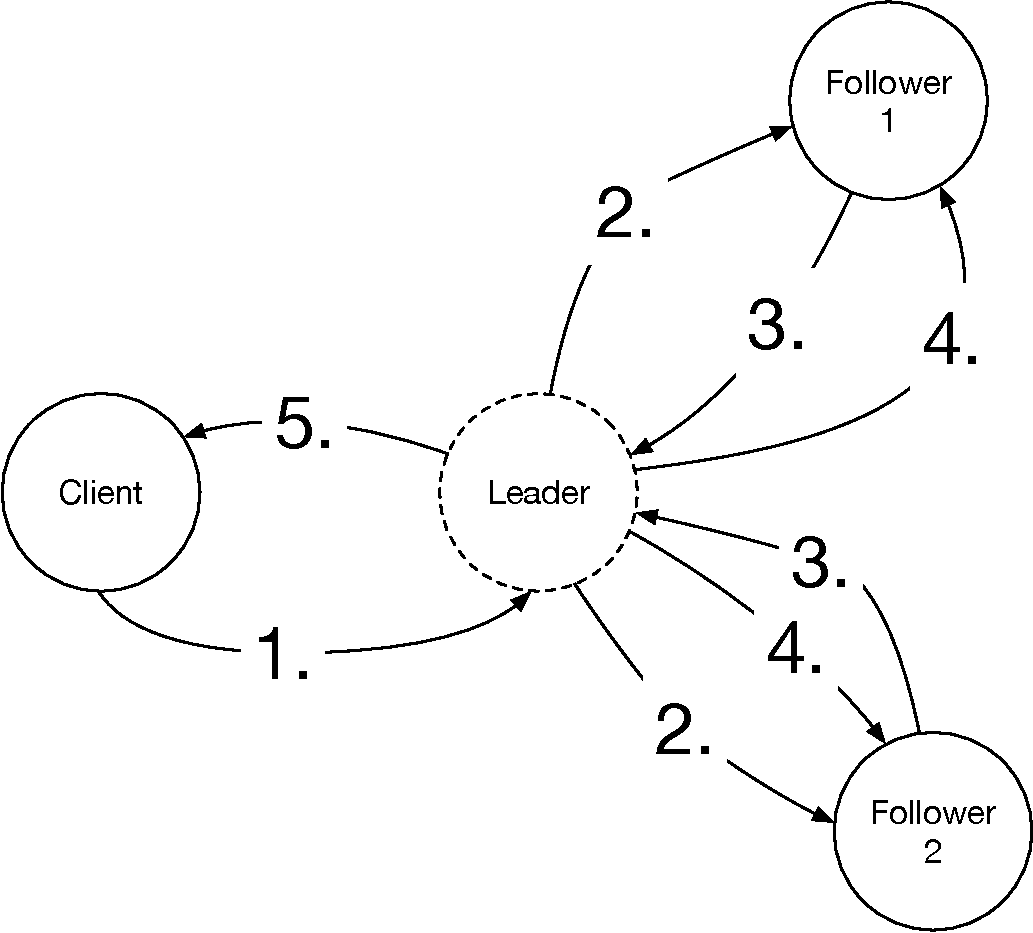
\includegraphics[width=0.8\textwidth]{client_server_interaction}
    \caption{Typical client server interaction for a replicated service call.
        Request arrives to the leader (1).
        Request is then replicated to all followers (2).
        Followers acknowledge the replication (3).
        Leader marks the request committed (4).
        Commited requests are forwarded to the application and reply is sent to the client (5).
        Note that all arrows are complete \gls{r2p2} messages: if they span multiple UDP datagrams, we wait for the complete message to arrive before replicating it.
    \label{fig:client-server-interaction}
    }
\end{figure}

Figure~\ref{fig:client-server-interaction} shows how a replicated request is handled.
In this example, the first node is the leader, and therefore the request must be directed to it (1).
The request is then packed in a log entry, and sent to the followers through Raft's \emph{AppendEntryRequest} message (2).
Nodes then send back an \emph{AppendEntryReply} message, acknowledging the message to the leader (3).
Once a request has been acknowledged by a majority of the nodes, the leader marks it as committed.
From this point on, the request will not be lost by the cluster\footnote{Provided that a majority of nodes stay healthy}.
Therefore, the request is forwarded to the application and the reply sent to the client (5).
On next message, or on timeout, the new commit index will also be sent to followers (4).
At this point they also forward it to their local copy of the application, which also sends back answers(5).
The replies sent from non-leader are silently dropped, as they would arrive after the leader's reply.

\chapter{Implementation}
\label{chap:implementation}

\section{Implementation language}

We initially planned to write the Raft prototype in Rust, using the NetBricks\cite{netbricks} framework.
The goal was to use Rust high level constructs to have compile time safety guarantees while maintaining good performance.
However, it turned out that using Rust for this project was less than ideal for several reasons.

NetBricks\cite{netbricks} is a Rust framework that provides everything needed to write high performance network applications in Rust.  % TODO: Something about Ogier writing R2P2 to rust
It provides a full userland networking stack, from the DPDK bindings up to UDP socket implementation.
Thanks to Rust's move semantics, NetBricks is capable of achieving zero copy processing of incoming packets, leading to very high performance.
Unfortunately, it does not appear to be developped actively anymore, which is an issue due to the fast evolving nature of the language.
The R2P2 Rust implementation\cite{ogier} written by another Master student appears to be incomplete at the moment.

Another issue with Rust was that the current ``reference'' implementation of R2P2 is written in C using a custom userland UDP/IP stack.
This means that the Rust / NetBricks code would have been difficult to integrate in the existing codebase, maybe even requiring a C rewrite.

Due to all those factors, we decided to switch the implementation strategy to directly writing code that could be used in C.
We use C++14, which is a lot more expressive than pure C.
Move semantics are also available in this language since C++11.
While not as useful as Rust's, mostly due to the lack of safety guarantees, they still form a very useful tool to reduce packet copying while simplifying memory management.

% TODO: Point to the fact that this could really be written in Rust, but maybe not using NetBricks (Ixy ?)

\section{Message serialization}

% TODO: is it really interesting ?

\begin{itemize}
    \item Custom code vs Protobuf
\end{itemize}



\section{Message Routing}
\label{sec:message_routing}

In Raft, only the leader can process new client requests.
This keeps the protocol simpler by only having data flowing from the leader to the followers.
On the other hand, it means that we must also have a way to direct client queries to the leader.

In the original Raft paper\cite{raft}, the followers will redirect clients to the leader if contacted directly.
However, this is not optimal from a tail latency perspective: a client that picks a follower as a destination will see an additional \gls{rtt} to its request.

Fortunately, \gls{r2p2} was implemented with load balancing semantics in mind.
We can therefore extend the \gls{r2p2} load balancer to always propagate replicated requests to the current leader.
While this haven't been done yet, it could be implementing by having the load balancer listening to Raft heartbeat messages (Figure~\ref{fig:r2p2_raft_routing}).

For our benchmarking we manually pointed the benchmark client to the elected leader.


\begin{figure}[h]
    \centering
    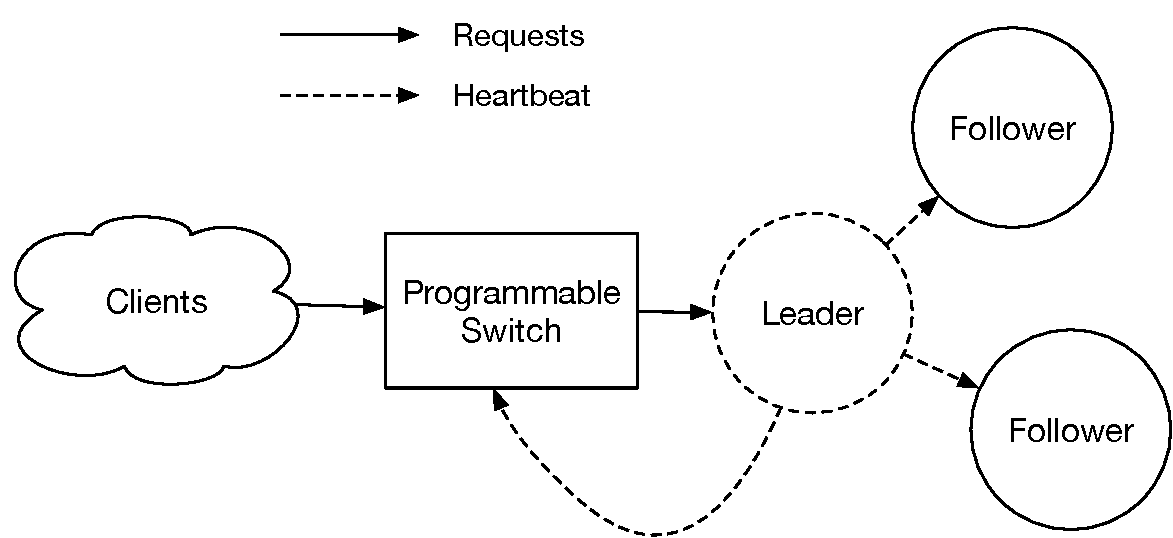
\includegraphics[width=0.8\textwidth]{r2p2_raft_routing}
    \caption{Message routing with R2P2 and Raft.
        The programmable switch listens to Raft leader heartbeats and forwards requests to the leader with the highest term.
    \label{fig:r2p2_raft_routing}
    }
\end{figure}

\section{Log}

At the end, Raft can only replicate a log, and ensure that all the nodes will eventually have all entries, in the same order.
We must provide an adequate definition of the log entries for our needs.
Since we are using Raft to replicate \gls{rpc} requests, the log entries will contain a \gls{r2p2} request: A source address and port, a request ID, and the request data.

To keep things simple and low latency, our log implementation stores its data in RAM only.
The requests are kept in a circular buffers, so that the oldest entry gets replaced by the newest one.
The data is stored into the circular buffer without copying; when an entry is overwritten, its data is given back to the network stack.

\section{DPDK backend}

In order to provide the best performance, \gls{r2p2} implements kernel bypass technologies.
In this mode, the application talks directly to a dedicated \gls{nic}, embedding the driver in the library code.

For the implementation we opted to use Intel's DPDK framework.
Several other kernel bypass framework exist such as netmap\cite{netmap}, or Ixy\cite{ixy}.
However they do not appear to have the same industrial traction as DPDK, neither are they cross platform; DPDK can run on Linux and FreeBSD on both Intel and ARM processors.

\section{Userland backend}

While kernel bypass offers the best performance, it is not always possible to use it (\ie when using a \gls{nic} is shared between applications).
Our current implementation can therefore either be compiled to use DPDK (and a custom UDP/IP stack) or to use the normal kernel networking facilities.
In this second case, only \gls{r2p2} is implemented in the application; the rest runs in-kernel.

To achieve high performance and stay close to DPDK's event based model, we use asynchronous I/O facilities.
Our first implementation used Linux's \texttt{epoll} directly, making it non-portable.
We rewrote it to use libuv instead, which abstracts the different asynchronous I/O mechanisms on Linux, BSD and Windows.

This means that the current implementation can run as a normal networked component on all major platforms.
This allows for a much easier development experience than running DPDK directly, and can even be used in production with good performance.

\section{Timers}

The Raft algorithm relies a lot on timers to detect leader absence and organize elections.
In order to implement this, we simply use the functions provided by both Intel's DPDK and libuv.
The port layer must only periodically call a function (\texttt{raft\_tick}).
This call is then used to process timeouts in various parts of the Raft implementation.

\section{Modification to client libraries}

The modification to client libraries are most of the time trivial.
Usually it is just setting the \gls{r2p2} routing policy to replicated.
The rest is then transparently handled by the server.

\chapter{Evaluation}
\label{chap:evaluation}

In this chapter, we measure the performance of our implementation.
In particular, we will focus on two key characteristics: latency and throughput.
Throughput is defined as the number of messages than can be succesfully replicated per second.
Latency is the time between the sending of a request and the reception of the reply (measured at the client).

We designed three different experiments to explore how our system reacts to different conditions.
In the first experiment, we measure the latency of a replicated operation under different fixed throughputs.
This will allow us to measure the peak throughput of the system, defined as the point at which the latency increases infinitely because requests are queued.
This experiment was carried using a cluster of three nodes.

In the second exeperiment, we measured the impact of cluster size on latency.
Since the leader must wait for a bigger quorum of machines to acknowledge the request, we expect the latency to go up with the number of machines.
We also include the case where there is only one machine in the group, i.e. when non replicated requests are used.
This was conducted at a fixed throughput.

For the last experiment, we wanted to measure the impact of leader failure on the system's throughput.
To do so, we modified the code of the server program to fall back to being a follower after a given number of messages was sent.
A new leader election would then take place and the requests sent while the cluster was leaderless would be lost.

All experiments were done on machines equipped with two Intel Xeon E5-2650 CPUs running at \SI{2.6}{\giga\hertz}.
Each machine had \SI{62}{\giga\byte} of RAM, out of which XXX were used for the application. % TODO: How many RAM for the app?
The machines were equipped with Intel~82599ES \glspl{nic} connected to a \SI{10}{\giga\bit\per\second} switch.
All the server machines were running the kernel bypass implementation of the stack, while the client was running the userland one.

\section{Latency - Throughput}

replicated vs non replicated

\section{Impact of cluster size}

at fixed load

\section{Latency over time}

including leader recovery

\section{Comparison with Kernel Paxos}

Kernel Paxos\cite{kernelpaxos} is an earlier attempts to reduce consensus protocol latency by removing the cost of context switching.
In order to do so, they implemented the Paxos protocol as a set of Linux kernel modules.
They had to port the libpaxos implementation, which was intended to run in userland, to things like kernel memory allocation.
Here are the main differences between their approach and ours:

\begin{itemize}
    \item Kernel Paxos is implemented as a set of Linux kernel modules.
        Our implementation uses Intel's DPDK\cite{dpdk} to access the \gls{nic} from userland.
    \item Kernel Paxos uses the Paxos algorithm.
        Our solution uses Raft.
    \item Kernel Paxos uses Ethernet frames to send its messages.
        This requires all machines to be in the same broadcast domain.
        Our implementation runs on top of UDP/IP and therefore can be routed.
\end{itemize}

The Kernel Paxos source code is freely available on the internet\footnote{\url{https://github.com/esposem/Kernel_Paxos}}.
Unfortunately we were not able to run it on our experimental setup.
Therefore, direct performance comparison might not be very accurate.
In particular, their node's CPU is much older than ours (2008 vs 2012).

\chapter{Conclusion}

We presented an extension to the \gls{r2p2} transport protocol that offers reliable, in-order, delivery of messages to application.
Our implementation uses well-known techniques like kernel bypass to offer both low tail latencies and high throughput.
We validated our design by running it against a series of microbenchmarks simulating different application workloads.
We observe an additional tail latency of only \SI{13}{\micro\second} compared to the unreplicated case.
On the throughput side, we only lose 14\% at a given \gls{slo}.
This shows that our original idea, moving consensus to the transport layer, can be both a general and high-performance tool for the distributed application developer. 

One key finding from this work is that latency of follower nodes matter a lot.
This means that application code should run on a separate thread on followers, to ensure the network code is not waiting on slow application requests.
We observed a throughput gain of up to 2x when implementing this separation of threads.

We believe that moving the consensus to the transport layer is the way to go for easy development of distributed applications.
However, before this solution can be used, there are some challenging issues to solve.
In particular, log compaction and persistent storage must be implemented to ensure true reliable consensus.
This could be a good extension to this project for a future master thesis.

\section*{Acknowledgements}

I would like to thank Marios Kogias for his help during all phases of this project.
Thank you also to the whole DCSL/VLSC team for the interesting lunch time discussion and teachings.


\nocite{*}
\bibliographystyle{ieeetr}
\bibliography{thesis}

\end{document}
